\documentclass[11pt]{article}
\usepackage[margin=1in]{geometry}
\usepackage{amsmath,amssymb,amsthm,mathtools}
\usepackage{graphicx}
\usepackage[hidelinks]{hyperref}
\usepackage{microtype}
\usepackage{xcolor}

\newtheorem{theorem}{Theorem}
\newtheorem{lemma}[theorem]{Lemma}
\newtheorem{corollary}[theorem]{Corollary}
\newcommand{\Hh}{\mathcal H}
\newcommand{\Ff}{\mathcal F}
\newcommand{\B}{\mathcal B}
\newcommand{\Ogl}{\mathcal O_{\mathrm{gl}}}

\title{Bounded Schauder matrices are path-connected, and\\
the unconditional orbit is not closed by basis type}
\author{Automated mathematics discovery run \texttt{fa\_banach\_001}\\
Lane 13, model GPT5.6}
\date{9 August 2026}

\begin{document}
\maketitle

\begin{center}
\fbox{\parbox{0.91\textwidth}{\textbf{Status.}
Candidate full solution, likely valid, subject to human review.  The first
theorem affirmatively answers Question 3.8 of the source.  The second theorem
gives a negative answer to Question 3.10, already when the starting matrix is
the identity (and hence unconditional).}}
\end{center}

\section{Source questions}

The source is Yang Cao, Geng Tian, and Bingzhe Hou,
\emph{Schauder Bases and Operator Theory III: Schauder Spectrums},
arXiv:1204.4232.  Fix an orthonormal basis $(e_n)$ of an
infinite-dimensional separable complex Hilbert space $\Hh$.  The paper calls
the matrix whose columns form a Schauder basis a \emph{Schauder matrix}.  In
Remark 3.7 it restricts to those matrices that represent bounded operators
and equips them with the operator-norm topology.  We denote this set by
$\Ff$.

Question 3.8 asks whether $\Ff$ is connected.  For $F\in\Ff$, the source
defines
\[
 \Ogl(F)=\{XF:X\in\mathrm{GL}(\Hh)\}
\]
and lets $\Ogl^c(F)$ consist of the Schauder matrices that are norm limits of
elements of $\Ogl(F)$.  Question 3.10 asks whether conditionality or
unconditionality must be preserved upon passing to $\Ogl^c(F)$.

\begin{figure}[h]
  \centering
  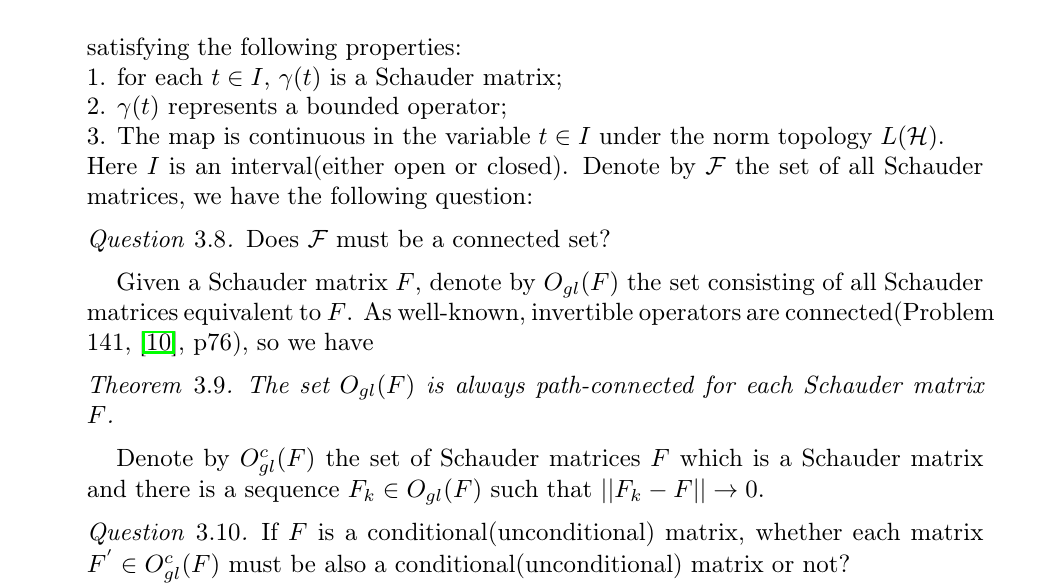
\includegraphics[width=0.98\textwidth]{figures/source_questions.png}
  \caption{Questions 3.8 and 3.10 on source PDF page 6.}
\end{figure}

\section{Proof intuition}

The source already observes that every bounded Schauder operator $T$ is
injective with dense range.  Therefore its polar decomposition
$T=U|T|$ has a \emph{unitary}, rather than merely partially isometric,
polar factor $U$.  Left multiplication by a unitary preserves the basis
property.  We can rotate $U$ continuously to the identity, leaving the
positive Schauder operator $|T|$.  The straight line from $|T|$ to the
identity is even simpler: except at its initial endpoint, every point on it
is positive and bounded below, hence invertible.  This joins every member of
$\Ff$ to the identity.

The same polar decomposition shows more.  For every $\varepsilon>0$,
$U(|T|+\varepsilon I)$ is invertible and is exactly $\varepsilon$ away from
$T$.  Thus \emph{every} bounded Schauder matrix lies in the closure of the
orbit of the identity.  Since bounded conditional Schauder matrices exist,
the closure of this unconditional orbit does not preserve unconditionality.

\section{Path-connectedness}

\begin{theorem}\label{thm:path}
The set $\Ff$ of bounded Schauder matrices on $\Hh$ is path-connected in the
operator norm.  More precisely, every $T\in\Ff$ can be joined to $I$ by a
norm-continuous path contained in $\Ff$.
\end{theorem}

\begin{proof}
Let $T\in\Ff$ and write its polar decomposition as
\[
 T=UA,\qquad A=|T|=(T^*T)^{1/2}.
\]
Because the columns $(Te_n)$ form a Schauder basis, $T$ is injective and has
dense range.  Hence $\ker A=\{0\}$, $\overline{\operatorname{ran}A}=\Hh$,
and the polar factor $U$ is unitary.  Moreover,
\[
 Ae_n=U^*Te_n,
\]
so $(Ae_n)$ is a Schauder basis: it is the unitary image of $(Te_n)$.

By the spectral theorem there is a bounded self-adjoint operator $B$ such
that $U=e^{iB}$.  Define, for $0\le t\le1$,
\[
 \gamma_T(t)=
 \begin{cases}
   e^{i(1-2t)B}A, & 0\le t\le\tfrac12,\\[2mm]
   (2-2t)A+(2t-1)I, & \tfrac12\le t\le1.
 \end{cases}
\]
The two formulas agree at $t=1/2$, and functional calculus makes the path
norm-continuous.  Also $\gamma_T(0)=UA=T$ and $\gamma_T(1)=I$.

For $0\le t\le1/2$, the operator $e^{i(1-2t)B}$ is unitary, so the columns
of $\gamma_T(t)$ are a unitary image of the Schauder basis $(Ae_n)$.
Consequently $\gamma_T(t)\in\Ff$.

For $1/2<t\le1$, put $s=2t-1>0$.  Since $A\ge0$,
\[
 (1-s)A+sI\ge sI.
\]
Thus $\gamma_T(t)$ is positive and boundedly invertible, and its columns
form a Riesz basis.  At $t=1/2$ the columns form the Schauder basis
$(Ae_n)$.  Hence the entire path lies in $\Ff$, proving the theorem.
\end{proof}

\section{The orbit-closure question}

\begin{theorem}\label{thm:closure}
For the identity Schauder matrix,
\[
 \Ogl^c(I)=\Ff.
\]
In particular, Question 3.10 has a negative answer: an unconditional
Schauder matrix can have a conditional Schauder matrix in the norm closure
of its equivalence orbit.
\end{theorem}

\begin{proof}
The inclusion $\Ogl^c(I)\subseteq\Ff$ is part of the definition of
$\Ogl^c(I)$.  Conversely, take $T\in\Ff$ and again write $T=UA$ as above.
For every $\varepsilon>0$, set
\[
 T_\varepsilon=U(A+\varepsilon I).
\]
The positive operator $A+\varepsilon I$ is boundedly invertible, as is
$T_\varepsilon$.  Therefore
\[
 T_\varepsilon\in\mathrm{GL}(\Hh)=\Ogl(I).
\]
Furthermore,
\[
 \|T_\varepsilon-T\|
 =\|U(A+\varepsilon I)-UA\|=\varepsilon.
\]
It follows that $T\in\Ogl^c(I)$ and hence $\Ogl^c(I)=\Ff$.

For completeness, we now exhibit a bounded conditional member of $\Ff$.
Let $(u_n)$ be any conditional Schauder basis of $\Hh$, and choose positive
numbers
\[
 \alpha_n=\frac{2^{-n}}{1+\|u_n\|}.
\]
The rescaled sequence $(\alpha_nu_n)$ is still a Schauder basis, with exactly
the same partial-sum projections as $(u_n)$, and is therefore conditional.
Define $S$ on the fixed orthonormal basis by
\[
 Se_n=\alpha_nu_n.
\]
Since
\[
 \sum_n\|Se_n\|^2\le\sum_n4^{-n}<\infty,
\]
$S$ is Hilbert--Schmidt and in particular bounded.  Thus $S\in\Ff$, and the
first part of the theorem gives $S\in\Ogl^c(I)$.  But $I$ is unconditional
whereas $S$ is conditional, which is the required counterexample.
\end{proof}

\section{Verification and scope}

The argument is internal to standard Hilbert-space operator theory.  The key
checks are:
\begin{enumerate}
  \item dense range makes the polar factor unitary;
  \item left unitary multiplication preserves all Schauder partial-sum
        projections up to unitary conjugacy;
  \item $(1-s)A+sI\ge sI$ for $A\ge0$ and $s>0$;
  \item $U(A+\varepsilon I)$ is invertible and converges to $UA$ in norm;
  \item diagonal rescaling by nonzero scalars does not change the partial
        sums of a Schauder expansion.
\end{enumerate}

The result concerns the bounded-operator class explicitly singled out in
Remark 3.7 and the norm topology used there.  It is stated for complex
Hilbert space, matching the source's spectral setting.  The counterexample
settles the preservation question negatively; it does not assert that the
closure of the orbit of every conditional basis contains an unconditional
basis.

\section{Novelty check}

The run's registry, solution, attempt, and proof-gap indexes were searched
for arXiv:1204.4232, the exact title, ``Schauder matrix'', connectedness, and
conditional orbit closure; no duplicate was found.  Bounded web searches on
9 August 2026 used the exact wording and numbering of Questions 3.8 and 3.10,
the paper title, and the authors.  They found the source and adjacent papers
on Schauder operators, but no later answer to either question.

The proof uses only the polar decomposition and a standard rescaling of a
conditional basis, so it may be folklore or an unnoticed immediate
consequence of known facts.  The novelty assessment is therefore
\emph{plausibly new as an explicit answer to these questions, moderate
confidence}.

\section{Human-review recommendation}

\textbf{Recommend priority review.}  The highest-value checks are that the
source's set $\Ff$ indeed fixes the same orthonormal coordinates along a path,
and that its notation $\Ogl^c(F)$ means relative norm closure among Schauder
matrices as transcribed above.  Under those definitions, both arguments are
short and exact.

\begin{thebibliography}{9}
\bibitem{CaoTianHou}
Y. Cao, G. Tian, and B. Hou,
\emph{Schauder Bases and Operator Theory III: Schauder Spectrums},
arXiv:\href{https://arxiv.org/abs/1204.4232}{1204.4232} (2012).

\bibitem{Singer}
I. Singer,
\emph{Bases in Banach Spaces I}, Springer, 1970.

\bibitem{Olevskii}
A. M. Olevskii,
\emph{On operators generating conditional bases in a Hilbert space},
Math. Notes \textbf{12} (1972), 476--482.
\end{thebibliography}

\end{document}
